\chapter{Theoretical background}
\label{ch:background} 
	\section{Web applications}
	%May be some more intro text''
		
	  Static HTML Web sites are loosing their popularity, because users
	  expect from modern Web sites more than just representing pictures and text.
	  Generally, users willing to have a higly responsive application with different useful
	  features, working in the web. As a result Web applications are displacing Web
	  sites on the market. The difference of Web application from a Web site is the
	 ``ability of a user to affect the state of the business logic on the
	 server"[7]. In other words the user/client makes a request to the server, the
	 server perform some actions (calculate, fetch data from database or external web-service) and
	  sends the response back to the client, which is rendered in the browser see
	  figure~\ref{fig:clientserver}.
	  \begin{figure}
	  \label{fig:clientserver}
      	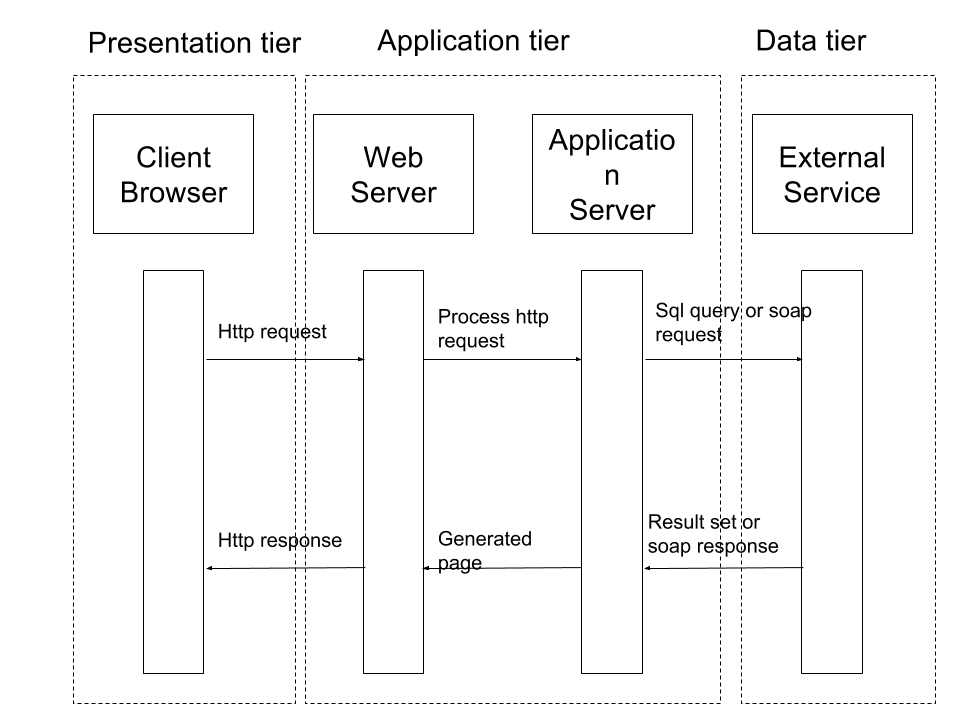
\includegraphics[width=0.75\textwidth]{client}
      	\caption{Web application structure}
      \end{figure}
	  
    	Client-server structure helps to distribute application tasks or workloads
    	between the service providers called servers, and service requesters, called
    	clients. Client-server model helps to separate client and server logic, as
    	a result these parts can be independent and communicate via application
    	programming interface (API). Client server model grants several advantages:
    	\begin{itemize}
    	  \item Client and server parts can be developed separately.
    	  \item The application may have several clients.
    	  \item Client, for example Web browser, is already created.
    	\end{itemize}
    		
    	Client server model is closely related to a multi-tier arhcitecture - the concept where
    	 the parts of the system are divided into separate tiers. Web applications
    	 are often user three-tier architecture:
    	 \begin{itemize}
    	   \item presentation tier is responsible for user interface generation and
    	   lightweight validation.
    	   \item application tier (business logic tier) controls an application
    	   functionality, determines how data is created, displayed, stored and
    	   changed.
    	   \item data tier - controls databases or other resources, provides access
    	   to the data.
    	 \end{itemize}
    	Multi-tier architecture allows any of the three tiers to be changed or
    	replaced independently, as a result developers have more freedom to use
    	external libraries and frameworks.
		
		All	applications have a lot of common features and problems which were already
		solved by developers beforehand. This is a good practise to take an already
		existing solution, than try to implement your own one. That is why many modern applications 
		are based on one or several software frameworks. The rapidly changing and
		highly competitive business environment, choosing a right toolset is one of the key factors of the sucess.
		Same implications are applied for testing frameworks. 	
		
		Nowadays some companies still rely on manual testing or ignore this
		important part of software development at all. Such approach has several
		sorrowful consequences:
		\begin{itemize}
			\item The developers are afraid of changing already written
			code. Because they do not have a confidence that their changes would not 
			break something. They stop cleaning their production code because they fear the
			changes would do more harm than good. ``Their production code began to rot"
			\cite[p.123]{cleanCode} 
			
			\item The effort of finding errors and	fixing them raises with the amount of code written.
			Because the developers can not localize the place where the error is actual
			happening.
			\item Developing new features become harder, if they are based on the part
			of the system which have errors.
		
			\item Cost increasing of the whole system.
	 	 \end{itemize}
	 	 
	 	 To test easily the huge amount of code an automated web testing is needed.	
	 	 Web testing reduces the amount of work requisite to check web applications as well as web sites, amplify software value, enhance
	 	 reusability of test cases and improve time-to-market.
	   
		IEEE has defined software testing as the process of evaluating a software
		system to verify that it satisfies specified requirements [3 XU]. A set of
		requirments for the web application includes security, performance,
		presentation, etc. We will focus on several requirements for the web
		application which differ from desktop application. 
		
		One of the key requirements which makes testing web applications harder than
		testing desktop applicatiosn is support of different browsers and operating systems and also
		different devices. A lot of desktop applications are developed to support some
		particular operating system or different versions of the product are developed
		and maintained for different operating systems. Web applications on the
		contrary should support not only different operating systems, but also
		different browsers and devices. So, if developers team decides to support
		three operating systems (Windows, OSX, Android), three type of devices (phone,
		tablet, PC) and three browsers (Chrome, Firefox, Internet Explorer) the number
		of possible variations is already twenty seven. If you decide to support
		different version of browsers, which in some circumstances may vary a lot,
		the number of different configurations of tested machines will be close to
		one hudred. In this case manual testing is unexceptable, because it will lead
		to unwarranted expenses. 
		
		Another difference between web and desktop applications is
		navigation on the webpage and between pages, the unexpected state change via
		the browser back button or direct Uniform Resource Locator(URL) entry in the
		browser. Also some resources or parts of the application can be not acccessable, due to
		connection problems or maintanance. Such unexpected behaviour may happen, and
		must be handled properly, not to crash the whole application.

		Web testing includes the different type of testing like:
		\begin{itemize}
		  \item functionality tests
		  \item compatibility tests
		  \item load tests
		  \item performance tests
		  \item integration tests
		\end{itemize}

		All these types of tests are equivalent important and picking a tool which
		will help to write these tests is not an easy task. It is an advantage when
		the testing tool is using same principles and similiar programming language
		with other tools in the project. We think that using same programming language
		to write both tests and code is much easier for the developer. This idea is
		related to Test-Driven Development(TDD), when tests are written
		before production code.
		
		TDD is a very popular methodology of software development. The main idea is to
		write tests first and then code. The main benefits of such approach are:
			\begin{itemize}
			  \item The developer is sure that his code works as intendent, because all his
				code is tested.
				\item The errors are found at early stage of the development cycle, which
				reduces the cost of fixing problems.
			\end{itemize}
			
			Three laws of TDD \cite[pp122]{Cleancode}[Book page 122]
				\begin{enumerate}
				  \item You may not write production code until you have written a failing unit	test.
				  \item You may not write more of a unit test than is sufficient to fail.
				  \item You may not write more production code than is sufficient to pass the
				curently failing test.
				\end{enumerate}
			\iffalse	
					\subsection {Approaches in Web Testing}	
						\begin{textit}
							In this chapter I will explain
							what does testing actually meands. What types of testing exist: unit, integration, user-interface, regression,
						etc. What are the differences between these types of testing.
						
						Next I will prove why testing is so important in software development. Here I
						would like to mention some information about \textit{Quality control}. The
						idea is to show that testing increseases the speed of software development
						and also improves it's quality. So in terms of quality control testing will
						decrease the price and increase the value of the product for the end user.
						
						Also I want to mention other methodologies like \textit{Agile development},
						\textit{User experience design} and \textit{Test Driven Development}. And how
						testing can be used/integrated with these methodologies/processes.
						\end{textit}
			\fi